\documentclass[extra,mreferee]{gji}
%\documentclass[extra]{gji}
\usepackage{timet}
\usepackage{amssymb}
\usepackage{amsmath}
\usepackage{graphicx}
\onecolumn

\title{Rapid and simultaneous estimation of fault slip and
  heterogeneous lithospheric viscosity from postseismic deformation}
\author[T.T. Hines and E.A Hetland]{T.T. Hines$^1$ and E.A. Hetland$^1$\\
                    $^1$ University of Michigan, 
                         Ann Arbor, MI, USA}
\date{Recived *; in original form *}
\pagerange{\pageref{firstpage}--\pageref{lastpage}}
\volume{*}
\pubyear{*}
\let\leqslant=\leq

\begin{document}

\label{firstpage}

\maketitle

\begin{summary}
\end{summary}

\begin{keywords}
\end{keywords}

\section{Introduction}
Geodetic observations of surface deformation in the months to years
following an earthquake are often attributed to afterslip
\citep[e.g.][]{M1991}, viscoelastic relaxation in the lithosphere
\citep[e.g.][]{NM1974}, and/or poroelastic-relaxation
\citep[e.g.][]{P1998,J2003}.  If postseismic deformation can be
entirely described by afterslip, then one could easily constrain the
spatial distribution of fault slip with a linear least squares
inversion \citep[e.g.][]{H1987,B2002,F2007}, which could then provide
insight into the frictional properties of faults
\citep[e.g.][]{H2006,B2009}.  However, postseismic deformation
following large ($M_w\geq$7) earthquakes is often attributed to
viscoelastic relaxation in the lithosphere
\citep[e.g.][]{HH2003,P2003,P2005} or a combination of both afterslip
and viscoelastic relaxation \citep[e.g.][]{F2006,H2008,J2009,R2015}.
In such cases, postseismic deformation can be used to constrain the
viscous properties of the lithosphere, although this is a more
difficult task than constraining a slip distribution.  Not only are
there potentially competing deformation mechanism which must be
discerned, finding the viscosity distribution of the lithopshere from
postseimsic deformation is a computationally expensive nonlinear
inverse problem.  Typically, this is approached with a forward
modeling, grid search method.  These forward modeling techniques
require the number of unknown parameters being estimated to be small,
meaning that significant and potentially inappropriate modeling
assumptions must be made \citep{RG2008,H2013}.

In this paper we propose a relatively fast method to kinematically
invert coseismic and postseismic deformation to simultaneously
estimate a time-dependent distribution of fault slip and an
arbitrarily discretized viscosity structure of the lithosphere.  Our
method is based on an approximation which linearizes the rate of early
postseismic deformation with respect to the viscosity of the
lithosphere.  We demonstrate the efficacy and limitations of our
method through a synthetic test.

\section{Linearizing early postseismic deformation} 
We assume that the lithosphere can be approximated as a Maxwell
viscoelastic material on the timescales of postseismic deformation,
where shear stress and strain are related by
\begin{equation}
  \frac{\partial\mitbf{\varepsilon}}{\partial t}=\frac{\mitbf{\sigma}}{2\eta} + 
                              \frac{1}{2\mu}\frac{\partial\mitbf{\sigma}}{\partial t}.
\end{equation}
$\eta$ and $\mu$ are viscosity and shear modulus, respectively.  This
constitutive relationship implies that a sudden strain in the
lithosphere from an earthquake will instantaneously propagate stresses
through the lithosphere elastically (assuming the lithosphere is
undergoing quasi-static deformation).  Creep will also initiate
immediately after the earthquake, where the initial viscous strain
rate in each parcel of the lithosphere will be proportional to the
fluidity ($\varphi=1/\eta$) in that parcel, and independent of the
fluidity elsewhere because stress at this time is only controlled by the
elastic properties of the lithosphere.  Each parcel will continue to creep at
approximately that rate for as long as the initial elastic stresses
from the earthquake are large compared to the stresses transferred
throughout the lithosphere by viscoelastic relaxation.  In this early
postseismic period, creep in each parcel will express itself as
surface deformation with an amplitude that is also proportional to the
fluidity in that parcel and independent of the fluidity elsewhere.
The early surface expression of creep in the entire lithosphere is
therefore a sum of the surface expression of each parcel and is linear
with respect to lithospheric fluidity.  This property of early
postseismic surface deformation is demonstrated below using simple
infinite length, strike-slip earthquake models, where the lithosphere
is approximated as a layered halfspace.  

\subsection{Two-dimensional earthquake models}
The easiest way to demonstrate how postseismic deformation can be
linearized with respect to lithospheric viscosity is with a
two-dimensional earthquake model consisting of a long, vertical,
surface rupturing, strike-slip fault that is embedded in a
viscoelastic horizontal layer overlying a viscoelastic halfspace.  We
make use of the correspondence principle of viscoelasticity
\citep[e.g.][]{F1975}, which states that the Laplace transform of
deformation in a viscoelastic body has the same form as the Laplace
transform of deformation in a elastic body with the same geometry and
subjected to the same boundary conditions. The solution for
displacements following an earthquake in a viscoelastic lithosphere
can then be easily found provided that the corresponding elastic
solution is known \citep[e.g.][]{NM1974,SP1978,HH2005}.  One only
needs to replace the shear modulus in the Laplace transform of the
elastic solution with the effective viscoelastic shear modulus and
then compute the inverse Laplace transform.

\subsubsection{Two layered model}
From the solution of \citet{R1971}, surface displacements,
$u_{e}(x,t)$, resulting from slip on a fault in an elastic surface
layer overlying a semi-infinite elastic substrate are
\begin{equation}\label{TwoLayerElastic}
  u_{e}(x,t) = b(t)\left(\frac{1}{2} W(0) + 
    \sum_{n=1}^\infty \Gamma^nW(n)\right),
\end{equation}
where
\begin{equation}
  W(n) = \frac{1}{\pi}\left(\tan^{-1}\left(\frac{2nH + D}{x}\right) 
    - \tan^{-1}\left(\frac{2nH - D}{x}\right)\right)
\end{equation}
and
\begin{equation}
  \Gamma = \frac{\mu_1 - \mu_2}{\mu_1 + \mu_2}.
\end{equation}
In the above equation, $b(t)$ describes cummulative slip on the fault
through time and can describe coseismic slip and/or afterslip. $D$ is
the locking depth of the fault, $H$ is the thickness of the upper
layer, and $\mu_1$ and $\mu_2$ are the shear modulii in the upper
layer and lower substrate, respectively.  The Laplace transform of eq
(\ref{TwoLayerElastic}) is
\begin{equation}\label{TwoLayerElasticLaplace}
 \hat{u}_e(x,s) = \hat{b}(s)\left(\frac{1}{2} W(0) +\sum_{n=1}^\infty\Gamma^nW(n)\right).
\end{equation}
We replace $\mu_1$ and $\mu_2$ in eq. \ref{TwoLayerElasticLaplace}
with the equivalent shear modulii for Maxwell materials in the Laplace
domain, $\hat{\mu}_1$ and $\hat{\mu}_2$, to get the Laplace
transform of surface displacements in the two-layered, viscoelastic
half-space,
\begin{equation}\label{TwoLayerViscousLaplace}
 \hat{u}_v(x,s) = \hat{b}(s)\left(\frac{1}{2}W(0) +\sum_{n=1}^\infty\hat{\Gamma}^nW(n)\right),
\end{equation}
where
\begin{equation}
  \hat{\Gamma} = \frac{\hat{\mu_1} - \hat{\mu_2}}{\hat{\mu_1} + \hat{\mu_2}}
\end{equation}
and
\begin{equation}
  \hat{\mu_i} = \frac{s}{\frac{s}{\mu_i} + \frac{1}{\eta_i}}.
\end{equation}
To find the surface displacements in the time domain one must find the
inverse Lapace transform of eq (\ref{TwoLayerViscousLaplace}), which
is typically done using the method of residues. However, we are interested in characterizing
the behavior of early postseismic deformation and it better serves us
to instead perform the inverse Laplace transform with an extension of
the initial value theorem (Appendix A). We assume for simplicity that
the shear modulus for the viscoelastic lithosphere is homogenous
(i.e. $\mu_1 = \mu_2$) and demonstrate in a supplementary IPython
notebook that our conclusions still hold when $\mu_1 \neq \mu_2$.  The
surface displacements in the time domain are
\begin{equation}
 u_v(x,t) = b(t)\frac{1}{2}W(0) + 
            b(t)\ast\mathcal{L}^{-1}\left[\sum_{n=1}^\infty\hat{\Gamma}^{n}W(n)\right].
\end{equation}
Evaluating the above inverse Laplace transform using the method
described in Appendix A, we find 
\begin{align}\label{TwoLayerViscous}
  u_v(x,t) = &b(t)\frac{1}{2}W(0) +\nonumber\\
             &b(t)\ast\left(\frac{\mu}{2\eta_2}W(1) - \frac{\mu}{2\eta_1}W(1)\right) +\nonumber\\
             &b(t)\ast\left(\left(\frac{\mu^2t}{4\eta_2^2} -
                  \frac{\mu^2t}{4\eta_1\eta_2}\right) \left(W(1) - W(2)\right) +
                  \left(\frac{\mu^2t}{4\eta_1\eta_2} - \frac{\mu^2t}{4\eta_1^2}\right)
                  \left(W(1) + W(2)\right)\right) + \nonumber\\ 
             &\dots.
\end{align}
The first term in eq (\ref{TwoLayerViscous}) is the elastic response
to slip on the fault.  The remaining terms describe the surface
displacement due to viscoelastic relaxation.  The first of these
remaining terms is the initial viscoelastic response and, as
suggested, it is a linear expression with respect to the fluidity in
each of the two layers.

If the time since the rupture is sufficiently small compared to the
relaxation times of each layer, $\tau_i=\eta_i/\mu$, (i.e. the third
and following terms in eq. (\ref{TwoLayerViscous}) are small), then we
can truncate the series and approximate early surface deformation
using only the elastic response and the initial viscoelastic response,
\begin{equation}\label{TwoLayerViscousApprox}
 u_v(x,t) \approx b(t)\frac{1}{2}W(0) + 
          \int_0^t b(\theta)\left(\frac{\mu}{2\eta_2}W(1) - 
                  \frac{\mu}{2\eta_1}W(1)\right)d\theta.
\end{equation} 
An approximation similar to eq. (\ref{TwoLayerViscousApprox}) was
demonstrated by \citet{S2010} for an elastic layer over a Maxwell
viscoelastic substrate.  

Figure 1 shows the series solution from eq. (\ref{TwoLayerViscous})
truncated at a sufficiently large $N$ along with the approximation
given by eq. (\ref{TwoLayerViscousApprox}). In this comparison, we use
$H=15$ km, $D=10$ km and a shear modulus of 32.0 GPa throughout the
lithosphere.  The upper layer is given a viscosity of $10^{20}$ Pa s
($\tau\approx 100$ years) and the substrate is given a viscosity of
$10^{19}$ Pa s ($\tau\approx 10$ years).  We let b(t) describe a unit
of instantaneous slip at $t=0.0$.  We find the that the approximate
solution is a good representation to the series solution for at least
as long as half the lowest of the two relaxation time, regardless of
our choice of model parameters.  The approximation breaks down faster
than what is show in Figure 1 when the upper layer is weaker than the
substrate or when we decrease the depth of the material interface
(i.e. when the weaker material is closer to the fault).  We also note
that the approximation has more longevity for locations further away
from the fault, where it starts to break down at about the minimum
relaxation time in the lithosphere.  Generally speaking, the timescale
over which eq. (\ref{TwoLayerViscousApprox}) accurately approximates
postseismic deformation is the same as the relaxation timescale of the
weakest region in the halfspace.

\subsubsection{Three layered model}
We follow the same procedure from above to find the surface
deformation resulting from slip on a strike-slip fault in a three
layered viscoelastic half-space.  Starting from the layered elastic
solution from \citet{CJ1972}, we evalutate the solution for the
viscoelastic problem in our supplementary IPython notebook.  We find
the initial viscoelastic response to a unit of slip to be
\begin{equation}\label{ThreeLayerViscousResponse}
\frac{\partial}{\partial t}u_v(x,t) = \frac{\mu}{2\eta_3}W(1,1)
                                      +\frac{\mu}{2\eta_2}(W(0,1) - W(1,1))
                                      -\frac{\mu}{2\eta_1}W(0,1),
\end{equation}
where
\begin{equation}
  W(n,m) = \frac{1}{\pi}\left(\tan^{-1}\left(\frac{2nH_2 + 2mH_1 + D}{x}\right) - 
                              \tan^{-1}\left(\frac{2nH_2 + 2mH_1 - D}{x}\right)\right).
\end{equation}
We see that eq. (\ref{ThreeLayerViscousResponse}) is once again linear
with respect to the fluidity in each of the three layers.  We can
approximate early postseismic deformation resulting from slip
described by $b(t)$ as
\begin{equation}\label{ThreeLayerViscousApprox}
u_v(x,t) \approx b(t)\frac{1}{2} W(0,0) + 
         \int_0^tb(\theta)\left(\frac{\mu}{2\eta_3}W(1,1)
                               +\frac{\mu}{2\eta_2}(W(0,1) - W(1,1))
                               -\frac{\mu}{2\eta_1}W(0,1)\right)d\theta,
\end{equation}
where $\eta_1$, $\eta_2$, and $\eta_3$ are the viscosities of the top,
middle, and bottom layers, respectively, and $H_1$ and $H_2$ are the
thicknesses of the top and middle layer, respectively.  We can see
that eq. (\ref{ThreeLayerViscousApprox}) recovers eq.
(\ref{TwoLayerViscousApprox}) when $\eta_3 = \eta_2$.

%It is worth noting that the initial viscoelastic response for the top
%layer, is equal and opposite in sign to the initial viscoelastic
%response from the underlying layers. In the context of an inverse
%problem, this means that it is impossible to use
%eq. (\ref{TwoLayerViscousApprox}) or eq. (\ref{ThreeLayerApprox}) to
%estimate the absolute viscosity of the each layers, rather it would
%only possible to estimate their relative viscosities. This is not a
%difficult obstacle to overcome because in application we can typically
%assume that the upper layer has a sufficiently long Maxwell relaxation
%time such that it is effectively elastic over the postseismic period.

\subsubsection{Continuous depth dependent model}
At this point we posit that a similar approximation can be made for an
arbitrarily layered lithosphere. In Appendix B we use
eq. (\ref{TwoLayerViscousApprox}) to find an initial viscoelastic
response kernel.  We then integrate that kernel over the depth of the
lithosphere to find the initial viscoelastic response for an arbitrary
depth dependent viscosity structure.  If the lithsophere is elastic
above the fault depth, $D$, and described by $\eta(z)$ below $D$ then
early postseismic deformation can be approximated as
\begin{equation}\label{ContinuousViscousApprox}
u(x,t) \approx \frac{b(t)}{\pi}\tan^{-1}(\frac{D}{x}) + 
               \int_o^t\int_D^\infty \frac{\mu b(\theta)}{2\pi\eta(z)}
                                    \left(\frac{2x}{x^2 + \left(D + 2z\right)^2} - 
                                    \frac{2x}{x^2 + \left(2z - D\right)^2}\right)
                                    dz d\theta.
\end{equation}
Although the above equation is capable of describing surface
deformation for an arbitrary depth dependent viscosity structure, it
falls short of being useful as the forward solution in an inverse
problem aimed at estimating lithospheric viscosity.  This shortcoming
is because the above equation makes the unphysical assumption that the
fault is infinitely long, in addition to the restriction of only being
applicable to a vertical strike-slip fault.  The assumption of
infinite length would introduce first order errors, which would likely
wash out the second order effect of viscosity. However,
eq. (\ref{ContinuousViscousApprox}) is useful for making estimates of
the depth sensitivity of postseismic deformation.

\subsection{arbitrarily discretized earthquake models}
Motivated by our above results, we make the assertion that the initial
rate of surface deformation resulting from an instantaneous
dislocation in a three-dimensional Maxwell viscoelastic
medium, which has been arbitrarily discretized into $N$ regions, will
have the form
\begin{equation}\label{PostseismicInitialVelocity}
  \frac{\partial}{\partial t}\vec{u}(\vec{x},t)\big|_{t=0} = \sum_j^N\frac{1}{\eta_j}G_j(\vec{x}).
\end{equation}
We denote $\vec{u}$ and $\vec{x}$ as vectors to emphasize that
eq. (\ref{PostseismicInitialVelocity}) is generalized to
three-dimensional problems.  We use $G_j(\vec{x})$ to represent the
initial rate of surface deformation at position $\vec{x}$ resulting
from viscoelastic creep in region $j$ with unit fluidity, where
fluidity is zero (i.e. elastic) in all other regions.  In this sense,
$G_j(x)$ can be thought of as a Green's function for the initial rate
of surface deformation resulting for viscoelastic deformation, and
thus we refer to $G_j(x)$ as the initial viscoelastic Green's
function.  We verify eq. (\ref{PostseismicInitialVelocity})
numerically in section 5.5 and save a theoretical justification for a
later paper.

Using eq. (\ref{PostseismicInitialVelocity}), we can then approximate
early surface deformation as
\begin{equation}\label{intermediate}
\vec{u}(\vec{x},t) \approx b(t)F(\vec{x}) + \sum_j^N\int_0^t
\frac{b(\theta)}{\eta_j}G_j(\vec{x}) d\theta,
\end{equation}
where $F(x)$ is the elastic Green's function, which describes the
elastic deformation resulting from a dislocation.  We further
generalize the approximation of surface deformation in
eq. (\ref{intermediate}) to allow for an arbitrary spatial
distribution of slip by using linear superposition.  If the elastic
defomation in a viscoelastic lithosphere can be described in terms of
$M$ elastic dislocation sources, then early surface deformation
resulting from both elastic dislocations and viscous creep can be
approximated as
\begin{equation}\label{Postseismic_Approximation}
\vec{u}(\vec{x},t) \approx \sum_i^Mb_i(t)F_i(\vec{x}) +
\sum_i^M\sum_j^N\int_0^t\frac{b_i(\theta)}{\eta_j}G_{ij}(\vec{x}) d\theta.
\end{equation}
The initial viscoelastic Green's function is dependent upon both the
region it represents as well as the dislocation source inducing
the viscoelastic creep in that region, hence the two indices.  It is
worth restating that the approximation given above does not account
for the viscoelastic coupling between the regions, since each region's
contribution to surface deformation is independent of the viscosity
elsewhere in eq.(\ref{Postseismic_Approximation}).  This approximation
is therfore appropriate for as long as the regions do not
significantly transfer stresses between eachother through viscoelastic
deformation.  Alternatively, since our initial viscoelastic Green's
functions do not have time dependence, one could view
eq. (\ref{Postseismic_Approximation}) as being appropriate up until
surface velocities resulting from viscous relaxation have decayed
appreciably.

\section{Inversion method}
The approximation of postseismic deformation given by eq.
(\ref{Postseismic_Approximation}) can be cast as an inverse problem
aimed at finding the distribution of slip on a fault and an
arbitrarily complicated lithosphere viscosity structure from
postseismic deformation. We assume that the slip history in any one
direction on each fault patch, $b_i(t)$, can be expressed as $P$ linear
terms such that
\begin{equation}
  b_i(t) = \sum_k^P \alpha_{ik}A_k(t),
\end{equation}
where $A_k(t)$ consists of either step functions describing coseismic
slip on a fault patch, or ramp functions, which have a constant, nonzero slope
over some time interval and are intended to represent afterslip.
The coefficient $\alpha_{ik}$ then represents either the amount of coseismic slip or
the cumulative slip over a time interval.  The approximation given by
eq. (\ref{Postseismic_Approximation}) now becomes
\begin{equation}\label{Postseismic_Approximation2}
  \vec{u}(\vec{x},t) \approx
  \sum_i^M\sum_k^P\alpha_{ik}F_i(\vec{x})A_k(t) +
  \sum_i^M\sum_j^N\sum_k^P\int_0^t\frac{\alpha_{ik}}{\eta_j}G_{ij}(\vec{x})A_k(\theta)d\theta.
\end{equation}
If we assume a fault geometry and the elastic properties of the
lithosphere, $F_i(\vec{x})$ can be computed with finite element
software or with an analytical solution
\citep[e.g.][]{O1992,M2007}. Likewise, $G_{ij}(\vec{x})$ can be
computed using finite element software.  If the assumed geometry of
the viscoelastic regions is sufficiently simple, $G_{ij}(\vec{x})$ may
also be computed with semi-analytic techniques
\citep[e.g.][]{P1997,FM2006,BF2010}.

We estimate the unknown slip parameters, $\alpha_{ik}$, and unknown
viscosities in each region of the lithosphere, $\eta_j$, from
observations of surface deformation in a least squares sense. Let
$\mitbf{u_{\mathrm{obs}}}$ be a vector of observed coseismic and postseismic
surface displacements at various locations and points in time.  Let
$\mitbf{m}$ be a vector of all the unknown parameters $\alpha_{ik}$
and $\eta_j$ with length $Q=M+N+P$, and let $\mitbf{u(m)}$ be a vector
of postseismic surface displacements predicted by eq
(\ref{Postseismic_Approximation2}). We seek to solve
\begin{equation}\label{Inverse_Problem}
  \mathrm{min}
  \big|\big|\mitbf{f(m)}\big|\big|_2^2
\end{equation}
subject to the constraint that
\begin{equation}
  \mitbf{m}\geq0,
\end{equation}
where 
\begin{equation}\label{ResidualFunction}
  \mitbf{f(m)} = 
    \begin{vmatrix}
      \mitbf{W\left(u(m)-u_{\mathrm{obs}}\right)}\\
      \lambda_s\mitbf{L_sm}\\
      \lambda_v\mitbf{L_vm}\\
    \end{vmatrix} .
\end{equation}  
In the above equation, $\mitbf{W}$ is a diagonal matrix containing the
reciprocal of the data uncertainties
(i.e. $\mitbf{W^TW}=\mitbf{C_d^{-1}}$ where $\mitbf{C_d}$ is
the data covariance matrix), and $\mitbf{L_s}$ and $\mitbf{L_v}$ are
regularization matrices.

We impose a nonnegativity constraint on $\mitbf{m}$ which ensures that
inferred slip is in one predominant direction and that viscosities are
positive.  Specifically, the rake of the inferred slip on each fault
patch is to be within a $90^\circ$ window defined by the rakes of
chosen orthogonal basis slip directions. For instance, the basis slip
directions could be chosen such that only slip rakes within $45^\circ$
of pure strike-slip, normal, or thrust are permisible.

Because this inverse problem inevitably has nonunique solutions for
$\mitbf{m}$, we put additional constraints on the inferred slip and
inferred viscosity with the matrices $\mitbf{L_s}$ and $\mitbf{L_v}$,
respectively.  In our following synthetic tests, we constrain the
solution by minimizing the Laplacian of the spatial distribution of
fault slip and lithospheric viscosity by letting
$\mitbf{L_s}$ and $\mitbf{L_v}$ be umbrella operators \citep{D1999}.
%such that they can be stacked on top of eachother into the matrix $L_{ij}$,
%which satisfies
%\begin{equation}
%  \sum_j^{Q}L_{ij}m_j = \frac{1}{|\mathcal{N}(i)|}\sum_{k\in \mathcal{N}(i)} m_k - m_i.
%\end{equation}
%In the above equation $\mathcal{N}(i)$ denotes the set of indices for
%model parameters describing slip (viscosity) which is adjacent to the
%slip (viscosity) described by $m_i$ and $|\mathcal{N}(i)|$ is the
%length of that set.
The parameters $\lambda_v$ and $\lambda_s$ in eq. (23) control how
much we enforce the smoothness constraint.  In our synthetic test, we
choose these parameters using L-curves, which describe the trade off
between the model smoothness and data misfit (Figure 2).  We first set
$\lambda_v=0$ and then use an L-curve to pick $\lambda_s=0$.  We then
fix $\lambda_s$ at our chosen value and use another L-curve to pick
$\lambda_v$.  We have attempted to choose our model parameters through
cross-validation but we found that the optimal pair of penalty
parameters picked through cross-validation tended to significantly
degrade our fit to the most near-field stations.

We find $\mitbf{m}$ that satisfies the above conditions using the
Gauss-Newton method \citep[e.g.][]{A2013}.  The best fit model parameters are
found by making an initial guess for the solution and then iteratively
solving
\begin{equation}\label{Gauss-Newton}
\mitbf{J}(\mitbf{m}^{k})\mitbf{m}^{k+1} = -\mitbf{f}(\mitbf{m}^k) + \mitbf{J}(\mitbf{m}^{k})\mitbf{m}^{k}
\end{equation}
for $\mitbf{m}^{k+1}$.  $\mitbf{J}(\mitbf{m}^k)$ is the Jacobian of
$\mitbf{f(m)}$ with respect to $\mitbf{m}$ evaluated at
$\mitbf{m^k}$. We impose the nonnegativity constraint on $\mitbf{m}$
by solving eq (\ref{Gauss-Newton}) with a nonnegative least squares
algoritm \citep{LH1974}. We find that it is occasionally necessary to
constrain the step size for each iteration of eq. (\ref{Gauss-Newton})
in order to ensure convergence.  We do so in a manner akin to the
Levenberg-Marquardt algorithm \citep[e.g.][]{A2013}.  We instead solve
\begin{equation}\label{Levenberg-Marquardt}
  \mitbf{J^*}(\mitbf{m}^k)\mitbf{m}^{k+1} = -\mitbf{f^*}(\mitbf{m}^k) + \mitbf{J^*}(\mitbf{m}^k)\mitbf{m}^k
\end{equation}
for $m^{k+1}$, where
\begin{equation}
  \mitbf{J^*}(\mitbf{m}) = 
      \begin{vmatrix}
      \mitbf{J}(\mitbf{m})\\
      \kappa\mitbf{I}
      \end{vmatrix},
\end{equation}
and
\begin{equation}
  \mitbf{f^*}(\mitbf{m}) = 
      \begin{vmatrix}
      \mitbf{f}(\mitbf{m})\\
      \mitbf{0}
      \end{vmatrix},
\end{equation}
and $\kappa$ controls the step size for each iteration and varies
depending on whether the algorithm is converging.  

In a nonlinear least squares algorithm, computing the Jacobian
typically is the largest computational burden; however, in this case
evaluating the Jacobian of eq. (\ref{Postseismic_Approximation2})
requires only a few computationally inexpensive matrix operations.
Consequently, our nonlinear least squares algorithm converges to a
solution for $\mitbf{m}$ in a matter of seconds on a desktop computer.
The main computational burden is in computing $F_i(x)$ and $G_{ij}(x)$
which is done with finite element software and only needs to be done
once for a given fault and lithosphere geometry. Throughout this
paper, our initial guess for the model parameters is that there is no
slip on any fault patch, and the lithosphere is entirely elastic
($1/\eta = 0$).  In our experience, the choice of initial guess has an
insignificant effect on the best fit solution.

\section{Synthetic test}
\subsection{Synthetic postseismic deformation}

We demonstrate with a synthetic test that our inverse method is
capable of recovering fault slip and lithospheric viscosity from
postseismic deformation.  We use the finite element software, Pylith
\citep{A2007}, to compute the surface deformation resulting from a
specified amount of slip on a fault in a lithosphere with a specified
viscosity.  We invert this synthetic surface deformation using the
method described above to recover the imposed model parameters.  The
synthetic test also serves to demonstrate that
eqs. (\ref{PostseismicInitialVelocity}) and
(\ref{Postseismic_Approximation}) are indeed valid for three
dimensional earthquake models.

Our synthetic model consists of a 50 km long by 20 km wide strike-slip
fault, striking to the north and dipping $60^{\circ}$ to the east (figure
4). At $t=0$ we impose $6.54*10^{19}$ N m of surface rupturing,
right-lateral coseismic slip with a distribution shown in Figure 3.
After the coseismic slip, we impose a constant rate of afterslip from
$t=0$ to 0.5 years.  The cumulative moment over this
interval is about $1.07*10^{19}$ N m.  The spatial distribution of
afterslip is shown in Figure 3.  During the interval $t=0.5$ to
1.0 years the rate of afterslip is decreased by a factor of 2.
We do not impose any fault slip beyond $t=1$ year.

The lithosphere in our synthetic model is Maxwell viscoelastic with
homogenous Lam\'e parameters $\lambda = 32$ GPa and $\mu = 32$
GPa.  The viscosity in the lithosphere decays from $10^{21}$ Pa s
($\tau\approx1,000$ years) at the surface to $10^{19}$ Pa s
($\tau\approx10$ years) at 75 km depth (Figure 4).  We compute
displacements at 0.1 year intervals up until $t=10$ years, which makes
the uppermost lithosphere effectively elastic on these timescales. We compute
surface displacements at 50 randomly chosen locations within a 400 km
square centered about the fault (Figure 5), which is intended to
roughly correspond with the density of GPS station at a well
instrumented plate boundary.  We add temporally correlated noise to
the computed displacements through time, consistent with what one would
expect from GPS observations.  The standard deviation of northing and
easting displacements is 1 mm, and the standard deviation of the
vertical displacements is 2.5 mm.  We add temporal covariance with an
exponential noise model that has a characteristic timescale of 0.25
years, which is intended to simulate seasonal processes that are
typically present in GPS time series.

\subsection{Green's functions}

We invert the synthetic surface deformation for fault slip on a 4 km
by 4 km discretization of the fault segment and we estimate a constant
viscosity in 10 km thick horizontal layers from the surface down to 70
km depth. We compute the elastic Green's functions, $F_i(\vec{x})$,
and initial viscoelastic Green's functions, $G_{ij}(\vec{x})$,
numerically using Pylith.  The elastic Green's functions are the
initial surface displacements resulting from 1 m of imposed slip on
fault patch $i$.  For each fault patch, we use basis slip directions
with rake $45^\circ$ updip and $45^\circ$ downdip of pure
right-lateral slip.  These slip basis directions restrict all inferred
slip to be within $45^\circ$ of right-lateral. We find the initial
viscoelastic Green's functions, $G_{ij}(\vec{x})$, by computing the
initial rate of surface deformation due to 1 m of slip on fault
patch $i$ in a model that is elastic everywhere except in region $j$,
which is assigned a viscosity of $10^{18}$ Pa s.

We define the basis slip functions, $A_k(t)$, as a heaviside function
centered at $t=0$ and three ramp functions which increase from 0 to 1
m of slip over the time intervals $t=0$ to $0.5$ years, $t=0.5$ to 1
year, and $t=1$ to 10 years.  Although our synthetic model does not
have any fault slip from $t=1$ to 10 years, we include the last
ramp function to test if postseismic deformation over that interval,
which is resulting purely from viscoelastic creep in the synthetic
model, can be describe with continued fault slip.

\subsection{Recovered model}

Our best fitting model of slip on the fault is shown in Figure 3.  The
spatial distribution and direction of inferred coseismic slip are a
good match to the synthetic coseismic slip.  The distribution of
afterslip was decently recovered but not as well as for the coseismic
slip.  There are a few artifacts in the distribution of afterslip
which are not present in the synthetic model, such as slip on the
north-most section of the fault.  The distribution of afterslip also
has been considerably smoothed out by the regularization. Our
inability to recover the details of the imposed afterslip as well as
the coseismic slip could be because the data noise is obscuring some
of the postseismic signal or possibly because the imposed afterslip is
deeper than the coseismic slip and thus more difficult to accurately
recover.  Nevertheless, the inferred moment of both coseismic slip and
afterslip, which is proportional to slip integrated over the fault
plane, is in good agreement with the moment in the synthetic model.
Although the spatial distribution of inferred slip may be more
difficult to recover, the cumulative slip seems to be consistently
recovered with ease.

The inferred slip over the last time interval, $t=1$ to 10 years, is
also consistent with the synthetic model.  The moment of slip
over this interval is $5*10^{17}$ N m, which is two orders of
magnitude smaller than the moment for the coseismic slip.  This means
that the inferred slip is accounting for, at most, a few mm's of
displacement from $t=1.0$ to $t=10.0$ years.  This is on order of the
data uncertainty and so the inferred slip is negligably small.  The
majority of surface deformation during this time interval is therefor being
properly attributed to viscoelastic relaxation.

The inferred viscosities in each of the eight layers are shown in
Figure 4a.  The recovered viscosities correspond well with the
synthetic model.  We used bootstrapping to estimate the uncertainties
of the recovered viscosities and we found that the strongest layers
near the surface, despite being proximal to the earthquake source,
have the highest uncertanties.  However, viscosities greater than
$~10^{20}$ Pa s are effectively elastic on the timescales of this
synthetic test and so a wide range of high viscosities for the upper
layers would just as adequately be able to describe the synthetic
surface displacements.  When looking at inferred values of fluidity
(Figure 4b), we see that the uncertainties are lowest at the surface
and increase with depth, as is perhaps more intuitive.

%We note that our inferred viscosities are strongly influenced by the
%regularization.  Indeed, many far less smooth viscosity structures
%would be able to fit the synthetic data just as well as what is shown
%in Figure 3.  Additionally, based on Figure 6, larger regularization
%parameters could have been used at only a slight cost to the models
%predictive power.  That is to say, an even smoother viscosity
%structure than that shown would also be able to adequately describe the
%synthetic data.

\subsubsection{Validation}
The fact that our recovered fault slip and lithospheric viscosity are
in good agreement with the synthetic model suggests that the
approximation given by eq. (\ref{Postseismic_Approximation}) is
accurate over the 10 years of synthetic data.  We further assess the accuracy
of eq. (\ref{Postseismic_Approximation}) by running a forward model
with Pylith where the imposed fault slip and lithospheric viscosity
are those estimated from the synthetic data.  We then compare the
displacements from the numerically computed forward model with the
displacements predicted by eq. (\ref{Postseismic_Approximation}).  We
refer to the numerically computed displacements as
$\vec{u}_{\mathrm{true}}(\vec{x},t)$ and the displacments predicted by our
approximation as $u(x,t)$ (Figure 6).  We refer to the
difference between $\vec{u}_{\mathrm{true}}(\vec{x},t)$ and $\vec{u}(\vec{x},t)$
as the approximation error (Figure 7). At $t=10$ years the
approximation error is on order of a few mm's in length for each
location, which is the magnitude of the data uncertainty.
Additionally, the approximation error is small compared to the
cm's of deformation resulting from viscoelastic relaxation, indicating
that eq. (\ref{Postseismic_Approximation}) is indeed a fair
approximation up to $t=10$ years.  

At $t=20$ years the approximation error is about
one cm in magnitude for near field sites, indicating that the
approximation has broken down in the near field by this time, while
the residuals are still on order of a few mm's for the far field
sites.  The faster divergence for the near field sites is consistent
with the comparison we made between the approximate and true
displacements for a two-dimensional, two layered earthquake model in
section 2.1.1 (Figure 1).

The accuracy of eq. (\ref{Postseismic_Approximation}) is also
demonstrated in Figure 6, which shows $\vec{u}(\vec{x},t)$ and
$\vec{u}_{\mathrm{true}}(\vec{x},t)$ at a sample site near the fault.  The
numerical solution asymptotically approaches the rate of deformation
predicted by eq. (\ref{Postseismic_Approximation}) as time goes to
zero, demonstrating that eq. (\ref{PostseismicInitialVelocity})
accurately descibes the initial viscoelastic response.  Additionally,
the magnitude of the difference between $\vec{u}(\vec{x},t)$ and
$\vec{u}_{\mathrm{true}}(\vec{x},t)$ is smaller than the uncertainty on our
synthetic data throughout the time series, indicating that the
approximation given by eq. (\ref{Postseismic_Approximation}) is
appropriate for this synthetic test.  For this site and other near
field sites, the approximation starts to break down at about $t=10$
years. The lowest relaxation time in our synthetic lithosphere is also
about 10 years and so the duration over which
eq. (\ref{Postseismic_Approximation}) is accurate is consistent with
our analysis for a two-dimensional, two layered earthquake model in
section 2.1.1.

%Figure 7 also shows the root mean square error as
%a function of time which we define as
%\begin{equation}
%  \mathrm{RMSE}(t) = \frac{\left|\left|\mitbf{u}(t) -
%    \mitbf{u}_{\mathrm{true}}(t)\right|\right|_2}{\sqrt{\mathrm{R}}},
%\end{equation}
%where R is the number of elements in $\mitbf{u}(t)$ and
%$\mitbf{u}_{\mathrm{true}}(t)$.  The root mean square error describes
%the average amount that the approximate displacements deviate from
%the true displacements for a given time.  The RMSE increases
%quadratically from 0 at $t=0$ to a few millimeters at $t=20$. 

\section{Discussion}

A fundemental assumption in our method for estimating slip and
viscosity from postseismic deformation is that the timescale of
relaxation in the weakest part of the lithosphere is at least as long
as the timescales over which postseismic deformation is observed.
This assumption allows us to approximate the surface expression of
viscous creep as a linear system with respect to lithospheric
fluidity, which greatly facilitates and expedites the inverse problem.
However, the lithosphere's relaxation time is generally not well
known.  There is then an added complication of deciding how much of
the postseismic time series to use in the inverse problem.  In our
synthetic example, we conveniently picked the length of our time
series to correspond with the weakest relaxation time in the
lithosphere. In general, the length of the postseismic time should be
determined iteratively in an inversion using our method.  For example,
if the approximation given by eq. (\ref{Postseismic_Approximation}) is
incapable of adequately describing observed postseismic deformation
or if inferred relaxation times are significantly less than the length
of the time series used in the inversion, then the time series should
be shortened.

%Talk about how inferred viscosity would change if the time series length is too long
our synthetic data is characterized by transient rapid postseismic
deformation in the first year after the earthquake followed by steady
deformation in the later years.  Surface deformation following large
($\geq M_w=7$) earthquakes often is characterized by a similar
temporal evolution \citep[e.g.][]{SS1997,S2005,E2009}.  Several
studies have attributed rapid early transience to afterlip and
described the later steady deformation with viscous relaxation in a
Maxwell viscoelastic lower crust or upper mantle
\citep[e.g.][]{PA2005,J2009,H2008,F2006,R2015}.  These studies have
found that lithospheric relaxation times no shorter than years or
decades are needed to describe postseismic deformation.  Indeed,
\citet{PA2005} descibed the trend in two years of postseismic
deformation following the 2001 $M_w=8.4$ Peru earthquake by assuming
that the lithospheric viscosity was sufficiently high that the rate of
deformation from viscoelastic creep could be considered constant,
which is the assumption that we make in formulating
eq. (\ref{Postseismic_Approximation}). If transient postseismic
deformation can be attributed to fault slip followed by steady
viscoelastic creep, then eq. (\ref{Postseismic_Approximation}) should
be appropriate on the timescale of years or decades after an
earthquake.

Several studies have explored other lithospheric rheologies to explain
observed transient postseismic deformation.  For example,
\citet{P2003,P2005} invoked a Burgers rheology upper mantle to explain
surface displacements following the 2002 $M_w=7.9$ Denali earthquake
and the 1999 $M_w7.1$ Hector Mine earthquake.  In both cases the best
fitting transient relaxation time was on the order of a month and the
best fitting steady state relaxation time was on the order of years.
Postseismic deformation following the Denali earthquake was also
successfully modeled by \citet{F2006b} with a power-law rheology in
the upper mantle, consistent with laboratory studies
\citep[e.g.][]{KK1987}.  The power-law rheology was able to reproduce
the observed transient surface deformation because the high stresses
in the earthquake decreased the effective viscosity of the upper
mantle to $~10^{17}$ Pa s resulting in fast surface deformation.  As
stresses from the earthquake relaxed, the effective viscosity
increased and the predicted surface deformation became steadier.

Based on the success of \citet{P2003,P2005} and \citet{F2006b}, one
may dismiss our method as being unrealistic because we assume that the
lithosphere is Maxwell viscoelastic.  However, our method does not
necessarily preclude the possibility of a Burgers rheology or a
stress-nonlinear viscosity.  As long as stresses in the lithosphere
remain roughly equal to the the stresses transferred elastically
through fault slip then a viscosity structure inferred using our
method could be interpretted as the effective viscosity for either a
Burgers rheology or a power-law rheology.  If the commonly observed
early transient postseismic deformation truly is the result viscous
relaxation in the lithosphere, then the results from
\citet{P2003,P2005} and \citet{F2006b} suggest that the time interval
over which eq. (\ref{Postseismic_Approximation}) is appropriate is on
order of a month after an earthquake.  Although one month of
postseismic data is a short window, such a low effective viscosity in
the upper mantle would yield a strong signal over this time.  We
postulate that the method described in this paper would then be able to
identify the location of the weak regions in the lithosphere with much
higher resolution than what could be obtained through the typical
forward modeling grid search method.  Any excised portion of the
timeseries could then be used to further constrain estimates of fault
slip and lithospheric viscosity by including it in a gradient based
nonlinear inverse method where the forward problem is computed
numerically rather that with eq. (\ref{Postseismic_Approximation}). In
such case, the initial guess for the model parameters would be the
estimates of slip and viscosity obtained from the truncated time series.


%talk about time stepping this algorithm?


\section{Conclusion}

\appendix
\section{Inverse Laplace transorm through series expansion}

let $f(t)$ be analytic at $t=0$ and let there
  be a real valued $M$, and $C$ such that
\begin{equation}\label{constraints}
  \left|f^{(n)}(t)\right| < Ce^{Mt}\quad \forall t\geq 0\text{ and }\forall n\in\{0,1,2,\dots\},
\end{equation}
where $f^{(n)}(t)$ denotes the $n^{th}$ derivative of $f(t)$.  We
define the Laplace transform of $f(t)$ as
\begin{equation}
  \mathcal{L}[f(t)] := \hat{f}(s) := \int_{0}^\infty f(t)e^{-st}dt
\end{equation}
and we restrict our attention to $s\in\mathbb{R}$.  The constraints on
$f^{(n)}(t)$ from eq. (\ref{constraints}) ensure that
\begin{equation}\label{Property2}
  \lim_{s \to \infty}\mathcal{L}[f^{(n)}(t)] = 0.
\end{equation}
It can be shown using integration by parts that
\begin{equation}\label{Property1}
  \mathcal{L}[f^{(n)}(t)] = s^n\hat{f}(s) - \sum_{m=1}^ns^{m-1}f^{(n-m)}(0)
  \quad \forall s>M.
\end{equation}
Substituting eq. (\ref{Property1}) into eq. (\ref{Property2}) and then
rearranging the terms gives us a recursive formula for $f^{(n)}(0)$ in
terms of $\hat{f}(s)$:
\begin{equation}\label{NthDeriv}
  f^{(n)}(0) = \lim_{s \to \infty} s^{n + 1}\hat{f}(s) -
               \sum_{m=1}^{n} s^{m}f^{(n-m)}(0),
\end{equation}
where the base case, $n=0$, is the initial value theorem:
\begin{equation}\label{NthDerivBase}
  f(0) = \lim_{s \to \infty} s\hat{f}(s).
\end{equation}
Since we request $f(t)$ to be analytic at $t=0$, we can construct a
Taylor series expansion of $f(t)$ such that
\begin{equation}\label{TaylorSeries}
  f(t) = \sum_{n=0}^\infty\frac{f^{(n)}(0)}{n!}t^n \quad \forall {t\in D},
\end{equation}
where $D$ is some neighborhood of $t=0$. We find the inverse Laplace
transform of $\hat{f}(s)$ for $t\in D$ by combining
eq. (\ref{TaylorSeries}) with eqs. (\ref{NthDeriv}) and (\ref{NthDerivBase}) so that $f(t)$ is
expressed in terms of $\hat{f}(s)$.

\section{Postseismic approximation for a two-dimensional earthquake model with an arbitrary depth dependent viscosity}
We seek to find an approximation for early postseismic deformation in
a two-dimensional, strike-slip earthquake model with an arbitrary
depth-dependent viscosity below the fault locking depth, $D$.  We
first find the initial rate of surface deformation following a unit of
slip in a lithosphere that is elastic except for a viscoelastic layer
which is at depth $z$ and with thickness $\Delta z$. This is found by
making the substitions $H_1 \to z$, $H_2 \to \Delta z$, $\eta_1 \to
\infty$, $\eta_3 \to \infty$, and $\eta_2 \to \eta$ in
eq. (\ref{ThreeLayerViscousResponse}), which gives us
\begin{equation}
  \frac{\partial}{\partial t}u_1(x,t)\big|_{t=0} = 
  \frac{1}{\eta}(W(z+\Delta z) - W(z)),
\end{equation}
where
\begin{equation}
  W(z) = \frac{\mu}{2\pi}\left(\tan^{-1}\left(\frac{2z-D}{x}\right) -
  \tan^{-1}\left(\frac{2z+D}{x}\right)\right).
\end{equation}
From eq. (\ref{PostseismicInitialVelocity}) we know that the initial
rate of surface deformation for a lithosphere composed of $N$ discrete
layers, each with viscosity $\eta_i$, at depth $z_i$, and having
thickness $\Delta z$, is then
\begin{equation}
  \frac{\partial}{\partial t}u_N(x,t)\big|_{t=0} = \sum_i^N
  \frac{1}{\eta_i}(W(z_i + \Delta z) - W(z_i)).
\end{equation}
The initial rate of surface deformation for a viscosity structure
given by $\eta(z)$ is found by taking the limit as $\Delta z \to 0$
and $N \to \infty$:
\begin{align}\label{ArbitraryViscousResponse}
 \frac{\partial}{\partial t}u(x,t)\big|_{t=0} &= \int_D^\infty
 \frac{1}{\eta(z)}\frac{\partial}{\partial z} W(z) dz\\
 &= \int_D^{\infty}\frac{\mu}{2\pi\eta(z)}\left(\frac{2x}{x^2 + \left(D + 2z\right)^2} -
                     \frac{2x}{x^2 + \left(2z - D\right)^2}\right) dz.
\end{align}
Finally, we add the elastic component of deformation and integrate
eq. (B.5) with the fault slip history to obtain
an approximation for early postseismic deformation:
\begin{equation}
u(x,t) \approx \frac{b(t)}{\pi}\tan^{-1}(\frac{D}{x}) + 
               \int_o^t\int_D^\infty \frac{\mu b(\theta)}{2\pi\eta(z)}
                                    \left(\frac{2x}{x^2 + \left(D + 2z\right)^2} - 
                                    \frac{2x}{x^2 + \left(2z - D\right)^2}\right)
                                    dz d\theta.
\end{equation}

\begin{thebibliography}{}

\bibitem[Aagard et al. (2013)]{A2007} Aagaard, B.T., Knepley, M.G. \&
  Williams, C.A., 2013. A domain decomposition approach to
  implementing fault slip in finite-element models of quasi-static and
  dynamic crustal deformation, \textit{J. Geophys.  Res. Solid Earth},
  118, doi: 10.1002/jgrb.50217.

\bibitem[Aster et al. (2013)]{A2013} Aster, R.C., Borchers, B.,
  Thurber, C.H., 2013. Parameter estimation and inverse problems,
  {\textit{Academic Press}}.

\bibitem[Barbot et al. (2009)]{B2009} Barbot, S., Fialko, Y. \& Bock,
  Y., 2009. Postseismic deformation due to the Mw 6.0 2004 Parkfield
  earthquake: Stress-driven creep on a fault with spatially variable
  rate-and-state friction parameters, \textit{J. Geophys. Res. Solid
  Earth}, 114, 1-26. doi:10.1029/2008JB005748.

\bibitem[Barbot \& Fialko (2010)]{BF2010} Barbot, S. \&
  Fialko, Y., 2010. A unified continuum representation of post-seismic
  relaxation mechanisms: Semi-analytic models of afterslip,
  poroelastic rebound and viscoelastic flow, \textit{Geophys. J.
    Int.}, 182, 1124-1140. doi:10.1111/j.1365-246X.2010.04678.x.

\bibitem[B\"urgmann et al. (2002)]{B2002} B\"urgmann, R.,
  Ergintav, S., Segall, P., Hearn, E.H., McClusky, S., Reilinger,
  R.E., Woith, H. \& Zschau, J., 2002. Time-dependent distributed
  afterslip on and deep below the \.Izmit earthquake rupture,
  \textit{Bull.  Seismol. Soc. Am.}, 92,
  126-137. doi:10.1785/0120000833.

\bibitem[Chinnery \& Jovanovich (1972)]{CJ1972} Chinnery,
  M.A. \& Jovanovich, D.B., 1972. Effect of earth layering on
  earthquake displacement fields, \textit{Bull. Seismol.  Soc. Am.},
  62, 1629-1639.

\bibitem[Desbrun et al. (1999)]{D1999} Desbrun, M., Meyer, M.,
  Schr\"oder, P. \& Barr, A.H., 1999.  Implicit fairing of irregular
  meshes using diffusion and curvature flow, \textit{Proceedings of
    the 26th Annual Conference on Computer Graphics and Interactive
    Techniques}, 317–324. doi:10.1145/311535.311576.

\bibitem[Ergintav et al. (2009)]{E2009} Ergintav, S.,
  McClusky, S., Hearn, E., Reilinger, R., Cakmak, R., Herrring, T.,
  Ozener, H., Lenk, O. \& Tari, E., 2009. Seven years of postseismic
  deformation following the 1999, M = 7.4 and M = 7.2,
  \.Izmit-D\"uzce, Turkey earthquake
  sequence. \textit{J. Geophys. Res. Solid Earth},
  114. doi:10.1029/2008JB006021.

\bibitem[Fl\"ugge (1975)]{F1975} Fl\"ugge,
  W., 1975. Viscoelasticity, Springer-Verlag Berlin Heidelberg.

\bibitem[Freed et al. (2006a)]{F2006} Freed, A.M., B\"urgmann,
  R., Calais, E., Freymueller, J. \& Hreinsd\'ottir, S.,
  2006. Implications of deformation following the 2002 Denali, Alaska,
  earthquake for postseismic relaxation processes and lithospheric
  rheology. \textit{J. Geophys. Res. Solid Earth}, 111,
  1-23. doi:10.1029/2005JB003894.

\bibitem[Freed et al. (2006b)]{F2006b} Freed, A.M.,
  B\"urgmann, R., Calais, E. \& Freymueller, J.,
  2006. Stress-dependent power-law flow in the upper mantle following
  the 2002 Denali, Alaska, earthquake, \textit{Earth
    Planet. Sci. Lett.}, 252, 481-489. doi:10.1016/j.epsl.2006.10.011.

\bibitem[Freed (2007)]{F2007} Freed, A.M., 2007. Afterslip
  (and only afterslip) following the 2004 Parkfield, California,
  earthquake, \textit{Geophys. Res. Lett.}, 34,
  1-5. doi:10.1029/2006GL029155.

\bibitem[Fukahata \& Matsu'ura (2006)]{FM2006} Fukahata, Y.,
  Matsu’ura, M., 2006. Quasi-static internal deformation due to a
  dislocation source in a multilayered elastic/viscoelastic half-space
  and an equivalence theorem. \textit{Geophys. J. Int.}, 166,
  418-434. doi:10.1111/j.1365-246X.2006.02921.x.

\bibitem[Harris \& Segall (1987)]{H1987} Harris, R.A. \&
  Segall, P., 1987. Detection of a locked zone at depth on the
  Parkfield, California, segment of the San Andreas
  Fault. \textit{J. Geophys. Res.}, 92,
  7945-7962. doi:10.1029/JB092iB08p07945.

\bibitem[Hirth \& Kohlstedt (2003)]{HK2003} Hirth, G. \& Kohlstedt,
  D.L., 2003. Rheology of the Upper Mantle and the Mantle Wedge : A
  View from the Experimentalists, \textit{Geophysical Monograph}, 138,
  83-105. doi:10.1029/138GM06.

\bibitem[Hearn et al. (2008)]{H2008} Hearn, E.H., McClusky, S.,
  Ergintav, S. \& Reilinger, R.E., 2009. \.Izmit earthquake
  postseismic deformation and dynamics of the North Anatolian Fault
  Zone. \textit{J.Geophys. Res. Solid Earth}, 114,
  1-21. doi:10.1029/2008JB006026.

\bibitem[Hetland \& Hager (2005)]{HH2005} Hetland, E.A. \& Hager,
  B.H., 2005. Postseismic and interseismic displacements near a
  strike-slip fault: A two-dimensional theory for general linear
  viscoelastic rheologies. \textit{J. Geophys. Res. Solid Earth}, 110,
  1-21. doi:10.1029/2005JB003689.

\bibitem[Hetland \& Hager (2003)]{HH2003} Hetland, E.A. \& Hager B.H.,
  2003. Postseismic relaxation across the Central Nevada Seismic Belt,
  \textit{J. Geophys. Res.}, 108,
  1–13. doi:10.1029/2002JB002257.

\bibitem[Hines \& Hetland (2013)]{H2013} Hines, T.T. \&
  Hetland, E.A., 2013. Bias in estimates of lithosphere viscosity from
  interseismic deformation, \textit{Geophys. Res. Lett.}, 40,
  4260-4265. doi:10.1002/grl.50839.

\bibitem[Hsu et al. (2006)]{H2006} Hsu, Y.-J., Simons, M., Avouac,
  J.-P., Galetzka, J., Sieh, K., Chlieh, M., Natawidjaja, D.,
  Prawirodirdjo, L. \& Bock, Y., 2006. Frictional Afterslip Following
  the 2005 Nias-Simeulue Earthquake, Sumatra, \textit{Science}, 312,
  1921-1926.


\bibitem[Johnson et al. (2009)]{J2009}Johnson, K.M.,
  B\"urgmann, R. \& Freymueller, J.T., 2009. Coupled afterslip and
  viscoelastic flow following the 2002 Denali Fault, Alaska
  earthquake. \textit{Geophys. J.  Int.}, 176,
  670-682. doi:10.1111/j.1365-246X.2008.04029.x.

\bibitem[J\'onsson et al. (2003)]{J2003} J\'onsson, S.,
  Segall, P., Pedersen, R. \& Bjornsson, G., 2003. Post-earthquake
  ground movements correlated to pore-pressure transients,
  \textit{Nature}, 424, 179-183. doi:10.1038/nature01758.1.

\bibitem[Kirby and Kronenberg (1987)]{KK1987} Kirby, S.H. \& Kronenberg,
  A.K., 1987. Rheology of the Lithosphere: Selected Topics. \textit{Rev.
  Geophys.}, 25, 1219-1244.

\bibitem[Lawson \& Hanson (1995)]{LH1974} Lawson, C.L. \&
  Hanson, R.J., 1995. Solving least Squares Problems, SIAM.

\bibitem[Marone et al. (1991)]{M1991} Marone, C.J., Scholz,
  C.H.  \& Bilham, R., 1991. On the mechanics of earthquake
  afterslip, \textit{J. Geophys. Res.}, 96, 8441-8452.

\bibitem[Meade (2007)]{M2007} Meade, B.J., 2007. Algorithms for the
  calculation of exact displacements, strains, and stresses for
  triangular dislocation elements in a uniform elastic half space,
  \textit{Computers and Geosciences}, 33,
  1064-1075. doi:10.1016/j.cageo.2006.12.003.

\bibitem[Nur \& Mavko (1974)]{NM1974} Nur, A. \& Mavko, G.,
  1974. Postseismic Viscoelastic Rebound, \textit{Science}, 183,
  204-206. doi:10.1126/science.183.4121.204.

\bibitem[Okada (1992)]{O1992} Okada, Y., 1992. Internal
  deformation due to shear and tensile faults in a half space,
  \textit{Bull. Seismol. Soc.  Am.}, 82, 1018-1040.

\bibitem[Peltzer et al. (1998)]{P1998} Peltzer, G., Rosen, P.,
  Rogez, F. \& Hudnut, K., 1998. Poroelastic rebound along the Landers
  1992 earthquake surface rupture. \textit{J. Geophys. Res.}, 103,
  30131-30145. doi:10.1029/98JB02302.

\bibitem[Perfettini et al. (2005)]{PA2005} Perfettini, H., Avouac,
  J.P. \& Ruegg J.C., 2005, Geodetic displacements and aftershocks
  following the 2001 Mw = 8.4 Peru earthquake: Implications for the
  mechanics of the earthquake cycle along subduction zones,
  \textit{J. Geophys.  Res. Solid Earth}, 110,
  1-19. doi:10.1029/2004JB003522.

\bibitem[Pollitz (1997)]{P1997} Pollitz, F.F.,
  1997. Gravitational viscoelastic postseismic relaxation on a layered
  spherical Earth. \textit{J. Geophys. Res.}, 102,
  17921-17941. doi:10.1029/97JB01277.

\bibitem[Pollitz (2003)]{P2003} Pollitz, F.F., 2003. Transient
  rheology of the uppermost mantle beneath the Mojave Desert,
  California, \textit{Earth Planet Sci. Lett.}, 215,
  89-104. doi:10.1016/S0012-821X(03)00432-1.

\bibitem[Pollitz (2005)]{P2005}Pollitz, F.F., 2005. Transient
  rheology of the upper mantle beneath central Alaska inferred from
  the crustal velocity field following the 2002 Denali earthquake,
  \textit{J. of Geophys. Res. Solid Earth}, 110,
  1–16. doi:10.1029/2005JB003672.

\bibitem[Riva \& Govers (2008)]{RG2008} Riva, R.E.M. \&
  Govers, R., 2009. Relating viscosities from postseismic relaxation
  to a realistic viscosity structure for the
  lithosphere. \textit{Geophys. J.  Int.}, 176,
  614-624. doi:10.1111/j.1365-246X.2008.04004.x.

\bibitem[Rollins et al. (2015)]{R2015} Rollins, C., Barbot,
  S. \& Avouac, J-P. 2015, Postseismic Deformation Following the 2010
  Mw7.2 El Mayor-Cucapah Earthquake: Observations, Kinematic
  Inversions, and Dynamic Models, \textit{Pure Appl. Geophys.},
  doi:10.1007/s00024-014-1005-6.

\bibitem[Rybicki (1971)]{R1971} Rybicki, K., 1971. The elastic
  residual field of a very long strike-slip fault in the presence of a
  discontinuity, \textit{Bull. Seism. Soc. Am.}, 61, 79-92.

\bibitem[Ryder et al. (2007)]{R2007} Ryder, I., Parsons, B.,
  Wright, T.J. \& Funning, G.J., 2007.  Post-seismic motion following
  the 1997 Manyi (Tibet) earthquake: InSAR observations and
  modelling, \textit{Geophys. J. Int.}, 169,
  1009–1027. doi:10.1111/j.1365-246X.2006.03312.x.


\bibitem[Savage \& Prescott (1978)]{SP1978} Savage, J. \&
  Prescott, W., 1978. Asthenosphere readjustment and the earthquake
  cycle, \textit{J. Geophys. Res.}, 83, 3369-3376.

\bibitem[Savage \& Svarc (1997)]{SS1997} Savage, J.C. \& Svarc, J.L.,
  1997. Postseismic deformation associated with the 1992 Mw=7.3
  Landers earthquake, southern California rupture,
  \textit{J. Geophys. Res.}, 102, 7565-7577.

\bibitem[Savage et al. (2005)]{S2005} Savage, J.C., Svarc, J.L. \& Yu,
  S.B., 2005. Postseismic relaxation and transient creep,
  \textit{J. Geophys. Res. Solid Earth}, 110,
  1-14. doi:10.1029/2005JB003687.1.

\bibitem[Segall (2010)]{S2010} Segall, P., 2010. Earthquake and
  volcano deformation, pp 185-186, Princeton University Press.



\end{thebibliography}

\begin{figure}[h!]\label{figure1}
  \centering
  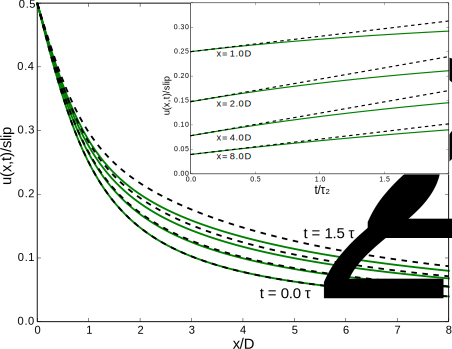
\includegraphics[width=0.8\textwidth]{FinalFigures/Figure1.pdf}
  \caption{Surface displacements predicted by
    eq. (\ref{TwoLayerViscous}) truncated after ten terms (green) and
    the approximation given by eq. (\ref{TwoLayerViscousApprox})
    (dotted black).  Times are normalized by the lowest relaxation
    time in the lithosphere, $\tau_2$, and distances are normalized by
    the fault locking depth, $D$.  Displacements are shown as a
    function of distance from the fault at times $t/\tau_2 =
    0.0,0.5,1.0$ and $1.5$. The inset figure shows displacement time
    series at locations $x/D = 1.0, 2.0, 4.0$ and $8.0$}
  \label{Figure 1}
\end{figure}

\begin{figure}[h!]\label{figure2}
  \centering
  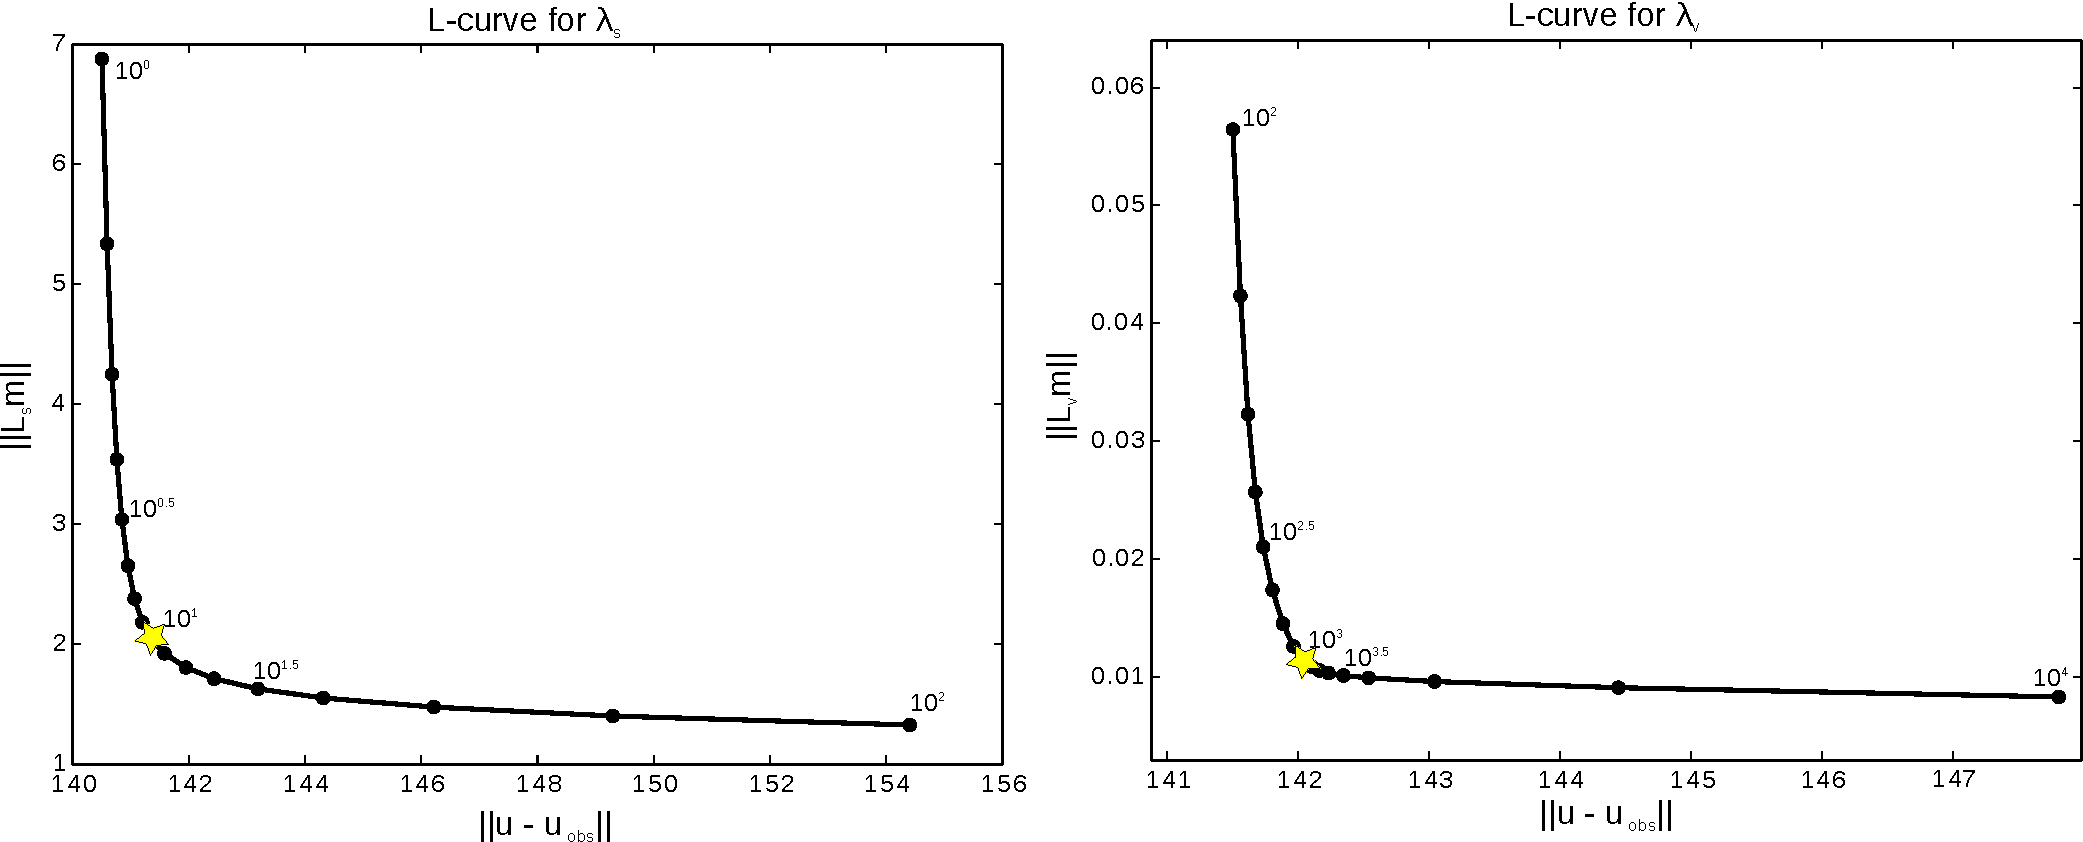
\includegraphics[width=0.9\textwidth]{FinalFigures/Figure6.pdf}
  \caption{L-curves used to select the penalty parameters. Panel A
    shows the trade off between slip smoothness and data misfit while
    varying $\lambda_s$ and keeping $\lambda_v$ fixed at zero.  Panel
    B shows trade off between smoothness of inferred viscosity and
    misfit while varying $\lambda_v$ and keeping $\lambda_s$ fixed at
    the value chosen from Panal A.  Stars indicate our chosen penalty
    parameters.}
  \label{Figure 2}
\end{figure}

\begin{figure}[h!]\label{figure3}
  \centering
  \includegraphics[width=0.9\textwidth]{FinalFigures/Figure2.pdf}
  \caption{Slip distribution imposed in the synthetic models and slip
    recovered from the inversion. Colors indicate magnitude of slip
    and arrows indicate direction of slip (arrows pointing right
    indicate left-lateral and up is thrust).  The panals showing
    afterslip display cumulative slip over the specified time
    interval.}
  \label{Figure 3}
\end{figure}

\begin{figure}[h!]\label{figure4}
  \centering
  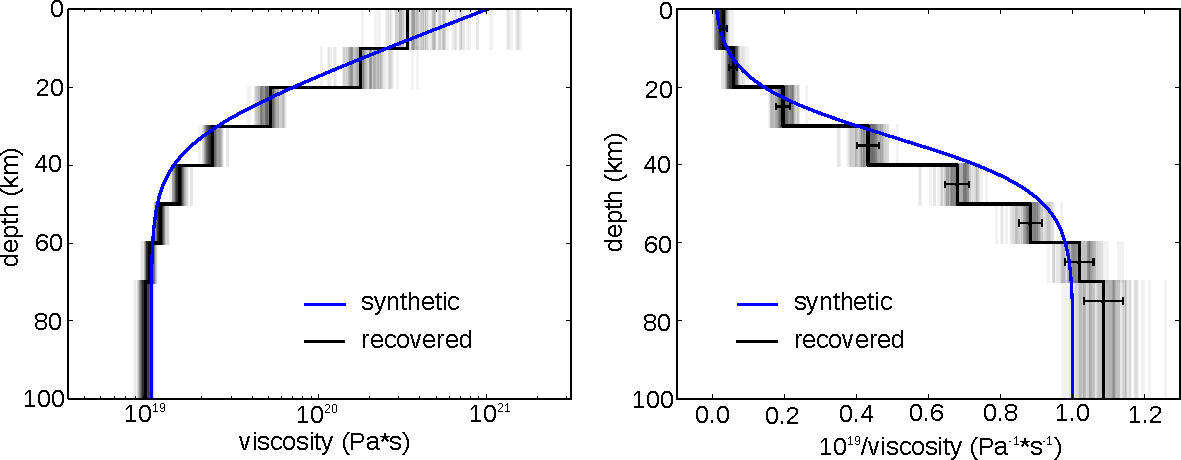
\includegraphics[width=0.9\textwidth]{FinalFigures/Figure3.pdf}
  \caption{Synthetic and recovered lithospheric viscosities (right)
    and associated fluidities (left).  Semi-transparent lines are recovered
    models found through bootstrapping and indicate the degree of
    uncertainty on the inferred viscosity structure.}
  \label{Figure 4}
\end{figure}

\begin{figure}[h!]\label{figure5}
  \centering
  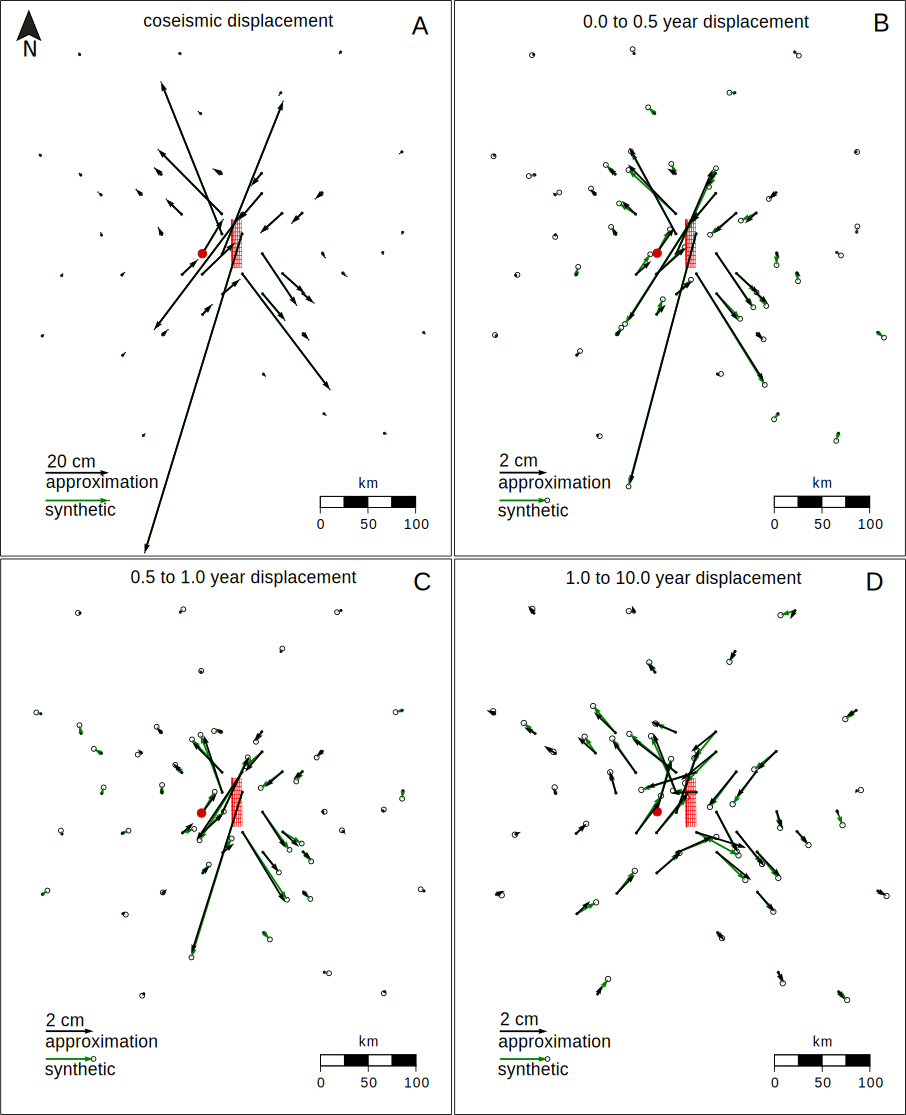
\includegraphics[width=0.9\textwidth]{FinalFigures/Figure4.pdf}
  \caption{Synthetic surface displacements (green) and best fitting
    surface displacements (black).  Vertical displacements are used in
    the inversion but are not shown here.  The top left panel shows
    coseismic displacements and the remaining panals show the
    cumulative displacements over the indicated time intervals. Red dot indicates
    the position of the time series shown in Figure 6. The surface
    projection of the discretized synthetic fault is depicted in red.}
  \label{Figure 5}
\end{figure}

\begin{figure}[h!]\label{figure6}
  \centering
  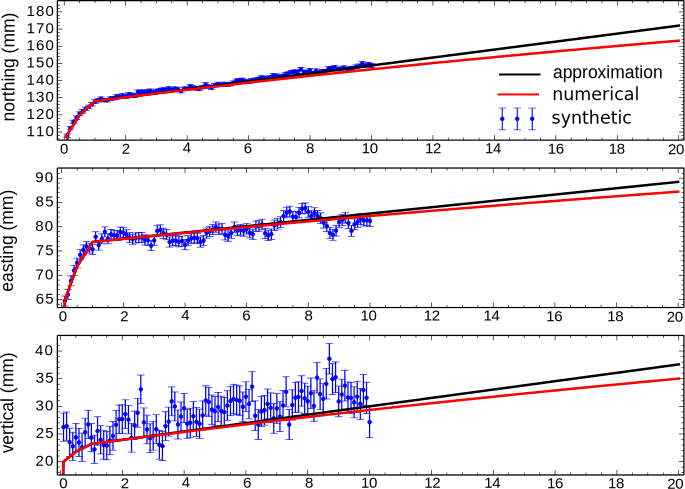
\includegraphics[width=0.9\textwidth]{FinalFigures/Figure5.pdf}
  \caption{Displacement time series for the position shown in Figure 5
    (green), best fitting surface displacements using the
    approximation from eq. (\ref{Postseismic_Approximation}) (black)
    and surface displacements computed with Pylith using the infered
    slip distribution and viscosity structure. Coseismic displacements
    at $t=0$ are not shown.}
  \label{Figure 6}
\end{figure}

\begin{figure}[h!]\label{figure7}
  \centering
  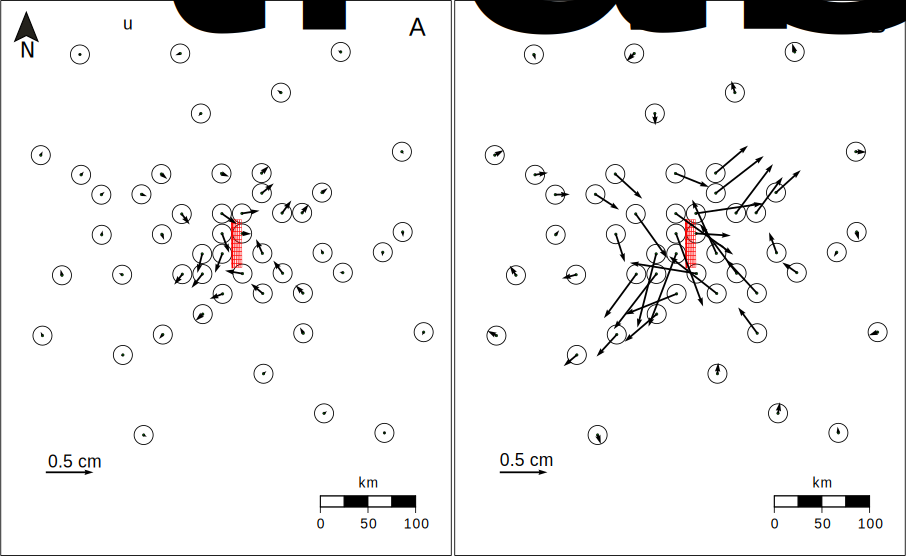
\includegraphics[width=0.9\textwidth]{FinalFigures/Figure7.pdf}
  \caption{Difference between $\vec{u}(\vec{x},t)$ and
    $\vec{u}_{\mathrm{true}}(\vec{x},t)$ at $t=10$ years and $t=20$ years.
    Circles with 1 mm radius are centered at each station to compare
    the accuracy of $\vec{u}(x,t)$ to the noise in
    the synthetic data.}
  \label{Figure 7}
\end{figure}


\end{document}
